% !TEX root = Master.tex

Simple maximum likelihood estimation based on the log-sales of the marginals allow us to estimate the exGaussian distribution parameters. \autoref{fig:kcc_2_marginal} describes how the histogram of the data match to the theoretical density of an exGaussian distribution considering the estimated parameter values represented in \autoref{tab:estimated_parameters_kcc_2_no_covariates}.
\\




\begin{table}[H]
\setlength\arrayrulewidth{1pt}  
\centering
\begin{adjustbox}{max width=\textwidth}\
\begin{tabular}{|c|c|c|}
\hline
\rowcolor{lightgray} 
$\hat{\mu}$ & $\hat{\sigma}$ & $\hat{\nu}$ \\ \hline
7.85        & 0.26           & 0.33        \\ \hline
\end{tabular}
\end{adjustbox}
\caption{Estimated parameters for log-sales of KCC 2 fitted to exGaussian distribution with no covariate effects}
\label{tab:estimated_parameters_kcc_2_no_covariates}
\end{table}





 \begin{figure}[H]
\centering
\begin{subfigure}{.45\textwidth}
  \centering
  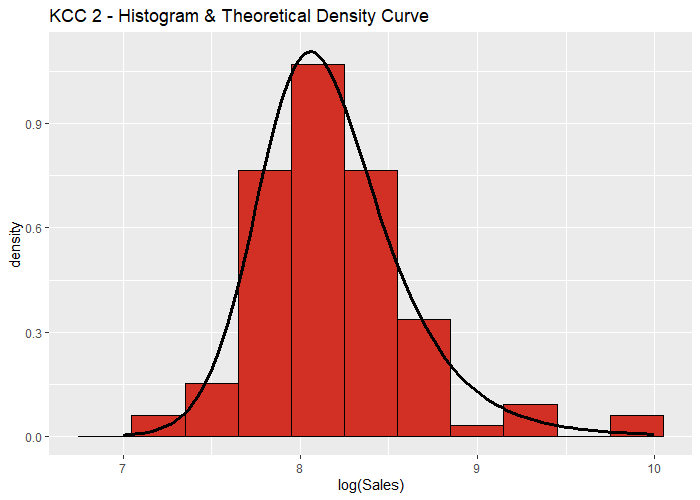
\includegraphics[width=\linewidth]{figures/kcc_2_density.png}
  \caption{Histogram \& theoretical density}
  \label{fig:kcc_2_density}
\end{subfigure}
\begin{subfigure}{.45\textwidth}
  \centering
  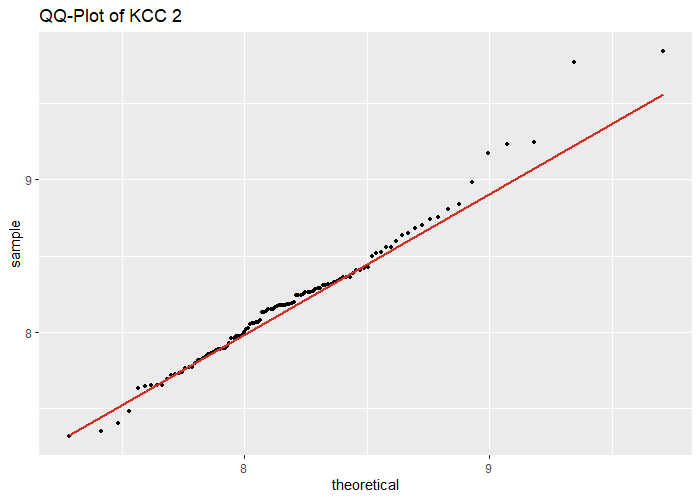
\includegraphics[width=\linewidth]{figures/kcc_2_qqplot.png}
  \caption{QQ-Plot}
  \label{fig:kcc_2_qqplot}
\end{subfigure}
\caption{exGaussian distribution fitted to log-sales of \ac{KCC} 2}
\label{fig:kcc_2_marginal}
\end{figure} 


As can be seen in \autoref{fig:res_kcc_2_no_covariates}, the residuals of the fitted distribution are not too far from a normal distribution. 
\\


\begin{figure}[H]
\centering
  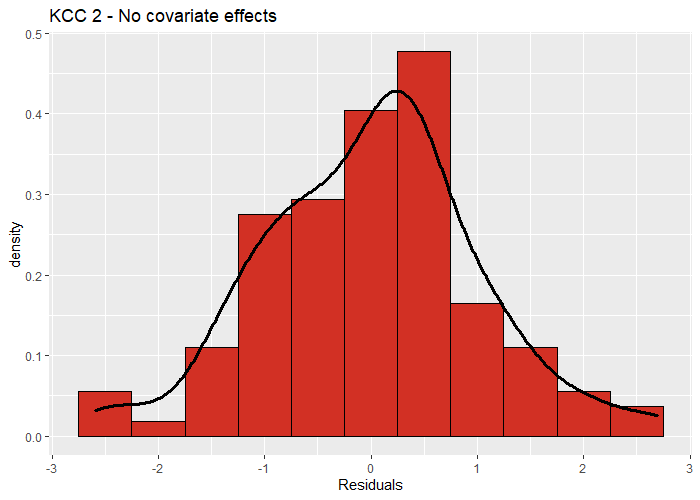
\includegraphics[width=0.45\linewidth]{figures/res_kcc_2_no_covariates.png}
  \caption{Residuals of KCC 2 log-sales fitted to an exGaussian distribution with no covariate effects together with a theoretical density curve of a normal distribution based on arithmetic mean and standard deviation}
  \label{fig:res_kcc_2_no_covariates}
\end{figure}

The findings so far indicate that the overall fit for this cluster are quite satisfiable and also support interpretability of the estimated parameters. \\

To make the estimation more precise and to get a better understanding of what is driving sales, flexible estimation of the distribution parameters is required and thus covariate effects shall be included. The temporal effects in particular are of special interest. 


